\documentclass[9pt,xcolor={dvipsnames}]{beamer}
\setbeamertemplate{navigation symbols}{}

\usetheme[progressbar=frametitle, block = fill]{metropolis}
%\usetheme[secheader]{Boadilla}
\usepackage{appendixnumberbeamer}
\usepackage[english]{babel}
\usepackage{booktabs}
\usepackage[scale=2]{ccicons}
\usepackage{array} % needed for \arraybackslash
\usepackage{graphicx}
\usepackage{adjustbox}
%\usepackage[utf8]{inputenc}
\usepackage{gensymb}
\usepackage{fourier}
\defbeamertemplate{itemize item}{compoundarrow}{\rule[0.5ex]{0.6ex}{0.6ex}%
	\scriptsize\raise2pt\hbox{$\!{\blacktriangleright}$}}
\makeatletter
\newcommand*{\indep}{%
	\mathbin{%
		\mathpalette{\@indep}{}%
	}%
}
\newcommand*{\nindep}{%
	\mathbin{%                   % The final symbol is a binary math operator
		%\mathpalette{\@indep}{\not}% \mathpalette helps for the adaptation
		\mathpalette{\@indep}{/}%
		% of the symbol to the different math styles.
	}%
}
\newcommand*{\@indep}[2]{%
	% #1: math style
	% #2: empty or \not
	\sbox0{$#1\perp\m@th$}%        box 0 contains \perp symbol
	\sbox2{$#1=$}%                 box 2 for the height of =
	\sbox4{$#1\vcenter{}$}%        box 4 for the height of the math axis
	\rlap{\copy0}%                 first \perp
	\dimen@=\dimexpr\ht2-\ht4-.2pt\relax
	% The equals symbol is centered around the math axis.
	% The following equations are used to calculate the
	% right shift of the second \perp:
	% [1] ht(equals) - ht(math_axis) = line_width + 0.5 gap
	% [2] right_shift(second_perp) = line_width + gap
	% The line width is approximated by the default line width of 0.4pt
	\kern\dimen@
	\ifx\\#2\\%
	\else
	\hbox to \wd2{\hss$#1#2\m@th$\hss}%
	\kern-\wd2 %
	\fi
	\kern\dimen@
	\copy0 %                       second \perp
}
\makeatother


\makeatletter
\newsavebox\myboxA
\newsavebox\myboxB
\newlength\mylenA

\newcommand*\xoverline[2][0.75]{%
	\sbox{\myboxA}{$\m@th#2$}%
	\setbox\myboxB\null% Phantom box
	\ht\myboxB=\ht\myboxA%
	\dp\myboxB=\dp\myboxA%
	\wd\myboxB=#1\wd\myboxA% Scale phantom
	\sbox\myboxB{$\m@th\overline{\copy\myboxB}$}%  Overlined phantom
	\setlength\mylenA{\the\wd\myboxA}%   calc width diff
	\addtolength\mylenA{-\the\wd\myboxB}%
	\ifdim\wd\myboxB<\wd\myboxA%
	\rlap{\hskip 0.5\mylenA\usebox\myboxB}{\usebox\myboxA}%
	\else
	\hskip -0.5\mylenA\rlap{\usebox\myboxA}{\hskip 0.5\mylenA\usebox\myboxB}%
	\fi}
\makeatother

%\usepackage[final]{pdfpages}

\makeatletter
\define@key{Gin}{foo}[]{\setkeys{Gin}{width=5in,height=3in}}
\makeatother


\usepackage{enumitem,amssymb}
\newlist{todolist}{itemize}{1}
\setlist[todolist]{label=$\square$}
\usepackage[retainorgcmds]{IEEEtrantools}
\setbeamertemplate{enumerate items}[ball]
%\usepackage[dvipsname]{xcolor}
\usepackage[geometry]{ifsym}
\usepackage{pgfplots}
\usepgfplotslibrary{dateplot}
\usepackage[]{natbib}
%\setcitestyle{authoryear, open={[[},close={)]}}
\usepackage{xspace}
\newcommand{\themename}{\textbf{\textsc{metropolis}}\xspace}
\usepackage[absolute,overlay]{textpos}
\usepackage{tikz}
\usetikzlibrary{matrix,chains,positioning,decorations.pathreplacing,arrows}
\usepackage[font={scriptsize}, labelfont = it]{caption}

%\usepackage{caption}
\captionsetup[figure]{labelformat=empty}% redefines the caption setup of the figures environment in the beamer class.

\usepackage{neuralnetwork}
%\usepackage[breaklinks,colorlinks]{hyperref}
\hypersetup{
	%citecolor=CornflowerBlue,naturalnames=true,hypertexnames=false,
	filecolor=magenta,      
	urlcolor=cyan,
	citecolor=blue,
}
\long\def\/*#1*/{}

\title{Extreme Value Theory :}
\subtitle{With Applications to Temperature Data}
\vspace{.5cm}
\date{\today}
\author{Antoine Pissoort \\ 
	\emph{Supervised by} Johan Segers\vspace{3ex}}
\institute{\emph{ISBA Universit\'e Catholique de Louvain}}
%\begin{center}
%	Universite Catholique de
%	Louvain
%\end{center}
% \titlegraphic{\hfill
\includegraphics[height=1.5cm]{logo.pdf}}
\defbeamertemplate{itemize item}{tikzarrow}{\tikz{\node[single
		arrow,scale=0.2,inner sep=2ex,fill] at (0,0) {};}}

\tikzset{
	myarrow/.style={
		draw,
		fill=Emerald,
		single arrow,
		minimum height=5.5ex,
		single arrow head extend=1ex
	}
}
\newcommand{\arrowright}{%
	\tikz [baseline=-1ex]{\node [myarrow,rotate=0] {};}
}

\newcommand{\backupbegin}{
	\newcounter{finalframe}
	\setcounter{finalframe}{\value{framenumber}}
}
\newcommand{\backupend}{
	\setcounter{framenumber}{\value{finalframe}}
}
\usepackage{appendixnumberbeamer}


\begin{document}
	\backupbegin
\maketitle

\begin{frame}{Table of contents}
	\setbeamertemplate{section in toc}[sections numbered]
	\tableofcontents[hideallsubsections]
	\thispagestyle{empty}
\end{frame}



\section{Introduction}

\backupend
\setbeamertemplate{footline}[frame number]
	
\begin{frame}
\frametitle{ Why do we need \boxed{\textbf{Extreme Value Theory}} ?}
\begin{block}{\textbf{A lot of applications in \textbf{various domains :}}}
	\begin{itemize}
		\item[$\bullet$] \textbf{Financial} : Risk analysis, insurance, stock fluctuations, $\dots$
	%	\item[$\bullet$] \textbf{Human wealth}
		\item[$\bullet$] \boxed{\textbf{Environmental}} most "important" application  :
		heatwaves, floods, drought, hurricanes, $\dots$
		\item[$\bullet$] $\dots$
	\end{itemize}
\end{block}
\begin{columns}[t]
	\begin{column}[]{.4\textwidth}
		\begin{textblock*}{4cm}(0.2cm,4.6cm) % {block width} (coords)
		\adjincludegraphics[width=\linewidth,valign=t]{evt1.pdf}
		\end{textblock*}
	\end{column}
	\begin{column}{.7\textwidth}
		$\Rightarrow$ \textbf{Extreme Value Theory} allows a relevant and efficient modelling of these \textbf{\textcolor{red}{extremes}} located at the \textcolor{red}{\textbf{tail}}(s) of the distribution.
		\begin{itemize}
			\item[$\bullet$] Low frequency of occurences (\textbf{small samples}) 
			\item[$\bullet$] Can be harder to grasp, to define, $\dots$
		\end{itemize}
		   $\Rightarrow$ large uncertainty

	\begin{todolist}
		\item \underline{2 main methods} :
		\begin{itemize}
			\item  $\Rightarrow$ \textbf{Block-maxima}
			 \item$\Rightarrow$ \textbf{Peaks-Over-}\textcolor{blue}{\textbf{Threshold}}
			 \item$\Rightarrow$ $\dots$
		\end{itemize}
	\end{todolist}
	\end{column}
\end{columns}
\end{frame}


\begin{frame}
\frametitle{\boxed{\textbf{Extreme Value Theory}} : Block-Maxima}
	Whereas $TCL$ deals with $\xoverline{X}$, we look here for a non-degenerate distribution in the limit for $X_{(n)}=\max(X_1,\dots,X_n)$.
	
	\begin{theorem}[\emph{Extremal Type} \textbf{from} Fisher-Tippett (1928)] Let $X_i\stackrel{iid}{\sim} F$ and let $a_n>0$, $b_n\in\mathbb{R}$ be sequences of constants, then 
 	\begin{equation*}
   \text{\emph{Pr}}\Big\{ a_n^{-1}(X_{(n)}-b_n)\leq z\Big\}=F^n(a_nz+b_n) \
   \longrightarrow G(z), \ \ \ \ \ \ \ \ n\to\infty.
	\end{equation*}
   where $G$ is a non-degenerate distribution function.
	\end{theorem}
	$G$ is known as the \emph{Generalized Extreme Value} ($GEV$) distribution :
	\begin{equation*}
	G(z)= \exp\Bigg\{-\bigg[1+\xi\bigg(\frac{z-\mu}{\sigma}\bigg)\bigg]^{\xi^{-1}}_+\Bigg\}.
	\end{equation*}
	\underline{3 parameters :} \ $\bullet$ \ $\mu \in\mathbb{R}$ : \emph{location} \ \ \ \ $\bullet$ \  $\sigma>0$ : \emph{scale} \ \ \ \ $\bullet$ \ $\xi\in\mathbb{R}$ : \textit{\textbf{\emph{shape}}}
\vspace{.2cm}

\begin{itemize}
	\item[$\triangleright$] Which block length ? (bias vs variance)
	\end{itemize}
\end{frame}


\begin{frame}
	\frametitle{\boxed{\textbf{Block-maxima}} method : 3 distributions }
	
\begin{columns}[c]
	\begin{column}{.7\textwidth}
%	\begin{figure}
	\centering
	\adjincludegraphics[width=\linewidth,valign=t]{gev.pdf}
	%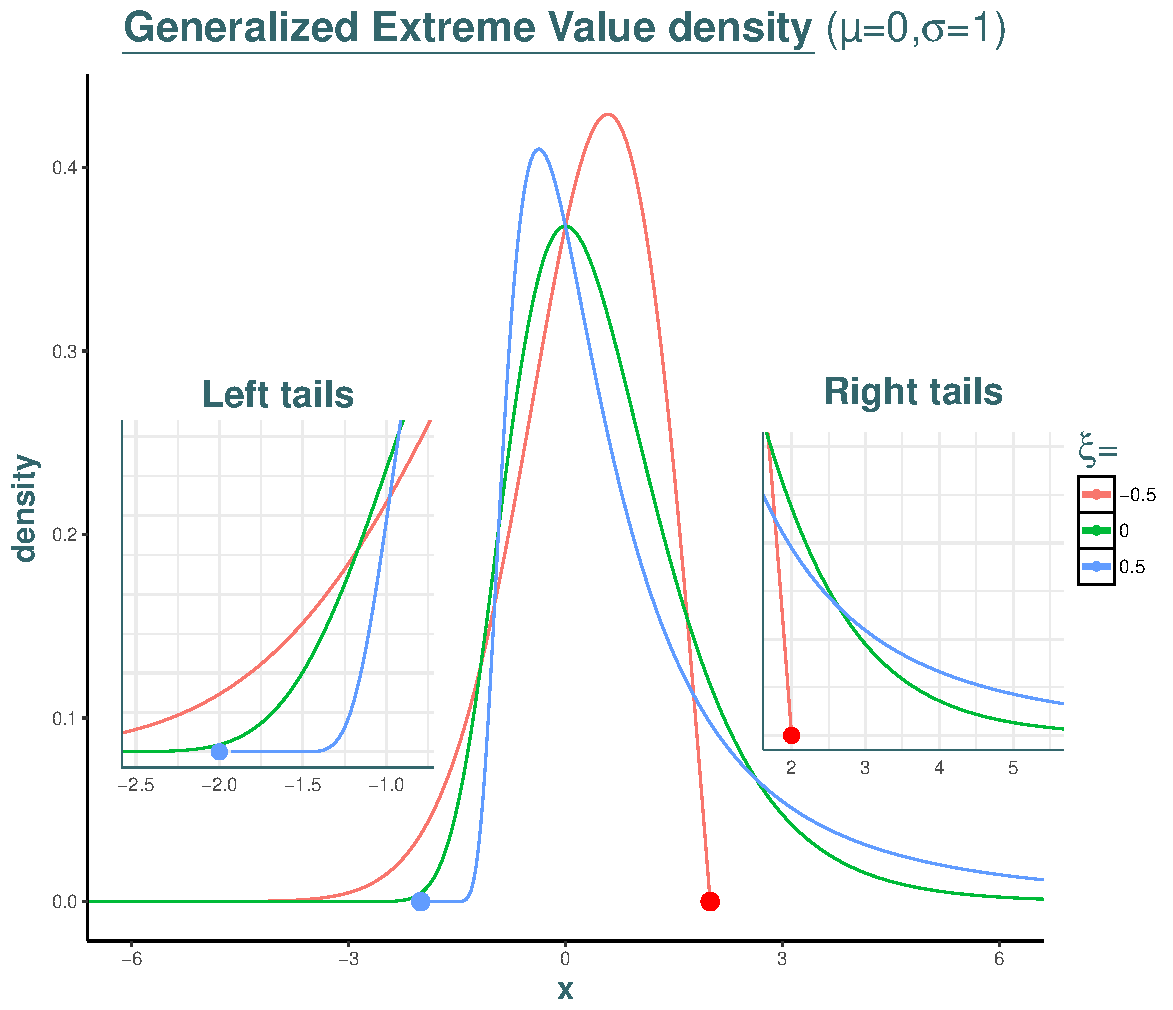
\includegraphics[width=3in, height = 2.5in]{gev.pdf}
	%\end{figure}
	\end{column}
	
   \begin{column}{.4\textwidth}

   		GEV distribution has 3 "child distributions" as special case
  \begin{block}{$\xi$ determines distribution }
\begin{itemize}
	\item[$\bullet$] \underline{\textcolor{red}{\textbf{Weibull}} family} : $\boxed{\xi<0}$ 
	right-endpoint, \\
	left heavy-tailed
	\item[$\bullet$] \underline{\textcolor{ForestGreen}{\textbf{Gumbel}} family }: $\boxed{\xi=0}$
	light-tailed
	\item[$\bullet$] \underline{\textcolor{blue}{\textbf{Fr\'echet}} family} : $\boxed{\xi>0}$
	left-endpoint,\\
	 right heavy-tailed
\end{itemize}
\end{block}
   \end{column}
\end{columns}
$\bullet$ \underline{E.g.} in our temperature data : $\xi\approx \textcolor{red}{-0.25}$ \ $\Rightarrow$ right-endpoint (why ?)
\end{frame}


 \begin{frame}
			\frametitle{\boxed{\textbf{Extreme Value Theory}} : Peaks-Over Threshold}
			Same principle as for block-maxima. But here, we don't look for only one value per block but  all values which exceed a fixed(?) threshold $u$.\\
			$\vartriangleright$ We deal now with the excess $\boxed{Y=X-u}$.  %$\boxed{H(y)=\text{Pr}\{X-u\leq y|X>u\}}$
\begin{theorem}[Pickands - Balkema - de Haan (1974)]  $X_i\stackrel{iid}{\sim} F$ and $x_*=\sup\{x:F(x)<1\}$ is the \emph{right-endpoint} of $F$. We have
\begin{equation*}
	\text{Pr}\big\{X-u\leq y\ |\ X>u\big\}=\frac{F(y+u)-F(u)}{\overline{F}(u)}\longrightarrow H_{\xi,\sigma_u}(y), \ \ \ \ \ \ \ \ \ \ u\to x_*,
	\end{equation*}
where $H$ is a (non-degenerate) Generalized Pareto Distribution (GPD).
			\end{theorem}
	
	\begin{columns}[T]\fontsize{7.5}{7}\selectfont
	\begin{column}{.6\textwidth}	We can easily prove it by the link with $GEV$ ($\dots$)
			\begin{equation*}
H(y)=
\renewcommand{\arraystretch}{0.6}\left\{\begin{array}{@{}l@{\quad}l@{}}
\ 1-\Big(1+\frac{\xi y}{\sigma_u}\Big)_+^{-\xi^{-1}}, \ \ \ \ \ \  \ \ \ \xi\neq 0; \\ 
\vspace{0.0002cm} \\
\ 1-\exp\Big\{-\frac{y}{\sigma_u}\Big\}, \ \ \ \ \ \ \ \ \ \ \ \xi=0.
\end{array}\right.\kern-\nulldelimiterspace
			\end{equation*}
			\newline
			Again, \underline{3 parameters :} \ $\bullet$ \ $\mu$ : \emph{location} \\ \ \ \ \ \ \ \ \ \ \ \ \ \ \ \ \ \ \ \ \ \ \ \ \ \ \ \ \
			 \ $\bullet$ \  $\sigma_u=\sigma+\xi(u-\mu)$ : \emph{scale}  \\
			 \ \ \ \ \ \ \ \ \ \ \ \ \ \ \ \ \ \ \ \ \ \ \ \ \ \ \ \ \ $\bullet$ \ $\boxed{\xi}$ : \textbf{\emph{shape}}
\end{column}
\begin{column}[t]{0.45\textwidth}
\begin{block}{\small $\boxed{\xi}$ determines distribution }
	\begin{itemize}
		\item[$\bullet$]\underline{"\textcolor{red}{\textbf{Beta}}" type} : $\boxed{\xi<0}$ 
		bound at $-\sigma/\xi$
		\item[$\bullet$] \underline{\textcolor{ForestGreen}{\textbf{Exponetial}} type }: $\boxed{\xi=0}$
		light-tailed
		\item[$\bullet$] \underline{\textcolor{blue}{\textbf{Pareto}} type} : $\boxed{\xi>0}$
		heavy-tailed
	\end{itemize}
\end{block}
\end{column}
			
\end{columns}
\end{frame}


\begin{frame}{Research Question(s) ?}
\begin{itemize}
\item[$\bullet$] "In-depth" study of univariate Extreme Value Theory (EVT)
\begin{itemize}
	\item[-] Characterization of main theoretical models/methods (see earlier)
	\item[-] Dealing with stationary and \textbf{non-stationary} sequences
\end{itemize}
\item[$\bullet$] Application of EVT to a new dataset gratefully delivered by the IRM : 
\begin{itemize}
	\item[-] Assess "\emph{Climate Change}" by trend analysis, extremes variability, $\dots$
	\item[-] Make relevant statistical inferences : Return Levels, $\dots$
\end{itemize}
\item\item[{\fontfamily{cyklop}\fontsize{6.5}{7}\selectfont \boxed{\textit{?}}}] Performance simulation study and comparisons of several "advanced" methods, effective in a \textbf{non-stationary} context : 
\begin{itemize}
	\item[-] Varying threshold selection methods:  \textbf{Mixture models}, $\dots$
	\item[-] \textbf{Bayesian} Analysis to better quantify uncertainty. Problem : \emph{prior} ?
	\item[-] \textbf{Neural Networks} : based on R library \texttt{GEVcdn}
	\item[-] \textbf{Bootstrap} evaluation to gain precision. \underline{E.g.:} confidence intervals
	\item[-] $\dots$
\end{itemize}

\end{itemize}
\end{frame}


\section{Literature Review}



\begin{frame}{ Literature Review : Main \boxed{\textbf{Books}}}\fontsize{7.9}{7.5}\selectfont
	\begin{block}{Basics for \emph{Extreme Value Theory}}
		\begin{itemize}
		\item[-]\textbf{\textcolor{JungleGreen}{\cite{coles_introduction_2001}}} \ $\rightarrow$ \ short \& very comprehensive
		\item[-] \textcolor{JungleGreen}{\cite{reiss_statistical_2007}} \ $\rightarrow$ \ more details \& statistical derivations
		\item[-]\textcolor{JungleGreen}{\cite{embrechts_modelling_2011}} \ $\rightarrow$ \ finance-insurance
oriented 		\item[-] \textcolor{JungleGreen}{$\dots$}
		\end{itemize}
	\end{block}
		\begin{block}{More (mathematically) strict and extensive} \begin{itemize}
			\item[-] \textbf{\textcolor{JungleGreen}{\cite{beirlant_statistics_2006}}} \ $\rightarrow$ \ big coverage + applications :\textbf{ time-series}
			\item[-] \textcolor{JungleGreen}{\cite{falk_laws_2011}}
			\item[-] \textcolor{JungleGreen}{\cite{haan_extreme_2006}}
		\item[-] \textcolor{JungleGreen}{$\dots$}
			\item[-] \textbf{\textcolor{JungleGreen}{\cite{dey_extreme_2016}}} \ $\rightarrow$ lots of research areas covered : \\ \textbf{non-stationarity}, \textbf{mixtures}, \textbf{bayesian},$\dots$
			\end{itemize}
		\end{block}
		\begin{block}{Climate-oriented}
		\begin{itemize}
			\item[-] \textcolor{JungleGreen}{\cite{mudelsee_climate_2014}} \ $\rightarrow$ \ + \emph{\textbf{bootstrap}} applications
			\item[-] \textcolor{JungleGreen}{\cite{aghakouchak_extremes_2012}} "in a \textbf{changing climate}" $\dots$\\
			 $\Rightarrow$ deals with \textbf{non-stationarity}
			 \item[-] \textcolor{JungleGreen}{$\dots$}
		\end{itemize}
		\end{block}

\end{frame}

\begin{frame}{ Literature Review : Main \boxed{\textbf{Articles}}}

Variety of interesting articles for each \textbf{part}, but mainly : 
\vspace{.3cm}
\begin{columns}
\begin{column}{.5\textwidth}

\begin{block}{(Advanced : multivariate)}
	\vspace{.1cm}
\centering	$\dots$ \vspace{.1cm}
	\end{block}

\begin{block}{Bayesian}
		\textcolor{JungleGreen}{\cite{stephenson_users_2006}} : for \texttt{\emph{evdbayes}} R package  \\
		\textcolor{JungleGreen}{\cite{northrop_cross-validatory_2017}} : Accounts for uncertainty in threshold selection \\ $\Rightarrow$ Bayesian model-averaging
\end{block}

\begin{block}{Climate - Neural Network}
 \textcolor{JungleGreen}{\cite{Galiatsatou_modeling_2016}} \\
  \textcolor{JungleGreen}{\cite{cannon_flexible_2010}}
\end{block}

\end{column}

\begin{column}{.5\textwidth}

\begin{block}{Bootstrap}
	
Wide applications, in many articles
\end{block}

\begin{block}{Stationary (clustering)}
	\textcolor{JungleGreen}{\cite{ferro_inference_2003}} :
\end{block}

\begin{block}{Non-stationary}
\textcolor{JungleGreen}{\cite{cheng_non-stationary_2014}} :
...
\end{block}

\begin{block}{Mixture Models}
	\textcolor{JungleGreen}{\cite{scarrott_review_2012}} : Review of available methods \\
	\textcolor{JungleGreen}{\cite{hu_extreme_2013}} : thesis on \texttt{\emph{evmix}} package
\end{block}

\end{column}

\end{columns}
\vspace{.5cm}
\centering $\dots \dots$ 
\end{frame}


\section{"Methodology" : Next Steps}


\begin{frame}{First Analysis of the \boxed{\textbf{Data}}}
\begin{columns}[c]
	\begin{column}{.5\textwidth}
		\centering
\adjincludegraphics[width=\linewidth,valign=t]{gg1.pdf}
	\begin{todolist}
		\item \textbf{TX} and TN in Uccle [1901-2016]
\small
		\item[$\bullet$] Upward trend : significant for all (TX, TN) but heavier for TX in summer
       \item[$\bullet$] \textcolor{cyan}{Trend} heavier in [1976-2016] than [1901-1975] : \textbf{climate warming}
	\end{todolist}
	\vspace{.4cm}
	\begin{todolist}
	\item We considered max(min) with (half-)yearly blocks. Also done with seasonal or monthly blocks
	\end{todolist}
	\end{column}

	\begin{column}{.6\textwidth}
	
	\centering
\adjincludegraphics[width=.99\linewidth,valign=t]{sumwint.pdf}
\newline
\newline
$\dots$ \quad $\dots$ \quad $\dots$
	\end{column}
 \end{columns}

\end{frame}

\begin{frame}\frametitle{Inference : First Methods}\fontsize{8.5}{9}\selectfont
	
	\vspace{1cm}
	\begin{columns}
		\begin{column}{.5\textwidth}
		\vspace{-.8cm}
\begin{block}{ Main Methods for GEV include}
\begin{itemize}
	\item[$\bullet$] \textbf{Maximum Likelihood} (ML) as usual is a good method but irregularities arise when $\xi<-0.5$

	\item[$\bullet$] \textbf{Penalized ML} : prior for $\xi$ to penalize values close to irregular region
\quad\item[$\blacktriangleright$] \textbf{\underline{Profile-likelihood}} : preferred in EVT due to the usual asymmetries in the likelihood surface of shape parameter

	\item[$\bullet$] \textbf{Moments} and \textbf{Probability-Weighted-Moments},$\dots$
\end{itemize}
\end{block}
		\end{column}
		\begin{column}{.5\textwidth}
				\vspace{-.8cm}
\begin{block}{ Main Methods for POT include}
	\begin{itemize}
		\item[$\ntriangleright$] \textbf{Hill} estimator ($\xi>0$)
		\item[$\bullet$] \textbf{Pickands}, \textbf{ML},$\dots$
		\item[$\blacktriangleright$] \textbf{Threshold selection }is an issue : \\ $\bullet$ for example look at \textbf{mean residual life} plot and check for linearity. \\
		$\bullet$ or vary threshold following seasons.
 	\item[$\blacktriangleright$] \textbf{Point Process} approach very useful : \\
 	unifies the 2 models and provides a natural formulation of non-stationarity in POT
	
	\end{itemize}
\end{block}
		\end{column}
\end{columns}

\begin{columns}
\vspace{-.5cm}
\begin{column}{.5\textwidth}
\begin{block}{Model diagnostics : Validation }
\underline{E.g.} check fit of the model by \textbf{PP} or QQ plot, \textbf{return level plot}, density, $\dots$ 
\quad \	\tiny \arrowright
\end{block}

\vspace{.2cm}
{\fontencoding{U}\fontfamily{futs}\selectfont\char 66\relax} Good fit but actually, data are not stationary... $\Rightarrow$ needs to handle this

\end{column}


\begin{column}{.5\textwidth}
	\vspace{.3cm}
\adjincludegraphics[width=\linewidth,valign=t]{pp_rl.pdf}
\end{column}

\end{columns}

\end{frame}


\begin{frame}{Relaxing Independence Assumption (1) : \boxed{\textbf{Stationary}} Extremes}
	
	\begin{block}{$D(u_n)$ condition : limited long-range dependence }
		In words, it says that if the $X_i$'s are not independent (most often) then provided the long-range dependence is limited, the extremal laws still occur in the limit.
	\end{block}
	
	\begin{block}{Theorem : Leadbetter (1983)}
	\small	Let $\big\{X^*_i\big\}$ be stationary series and $\big\{X_i\big\}$ be iid series of $n$ R.V.'s. Then, we have that 
	\normalsize
   \begin{equation*}
	\text{Pr}\big\{a_n^{-1}(X_{(n)}-b_n)\leq x\big\}\longrightarrow G(x), \ \ \ \ \ \ \ n\rightarrow \infty
   \end{equation*}
\ \ \ \ and  \ \ \ \ \ \ \ \ \quad 
   %\text{and} %\hspace{1.3cm} 
 %  \ \ \ \ \ \ \ \ \ \ \ \ \ \ \ \ \ \ \ \ \
   	$\text{Pr}\big\{a_n^{-1}(X^*_{(n)}-b_n)\leq x\big\}\longrightarrow G^*(x), \ \ \ \ \ \ n\rightarrow \infty$

\ \ \ \ where  \ \ \ \ \ \ \ \ \ \ \ \ \ \ \ \ \ \ \ \ \ \ $G^*(x)=G^{\theta}(x).$
	\end{block}
	\vspace{-.2cm}
	$\boxed{\theta}$ is the \textbf{extremal index} which quantifies the extent of extremal dependence
	\begin{columns}[T]
		\begin{column}{.6\linewidth}\fontsize{7.5}{7}\selectfont
	\vspace{-1.5mm}
\begin{itemize}
	\setbeamertemplate{itemize item}[triangle]
	\item[$\vartriangleright$] Parameters of $G^*$ and $G$ are related
	
	\vspace{.25cm}
\end{itemize}
{\fontencoding{U}\fontfamily{futs}\selectfont\char 66\relax} POT : \textbf{Clusters of extremes} with mean size $\theta^{-1}$

For threshold of $30^{\circ}c$ : we obtain $\boxed{\theta\approx 0.5}$ \ $(\nindep)$ \ \ \ \    \arrowright \\
 \vspace{.33cm}
 $\Longrightarrow$ Needs for \textbf{declustering} (e.g. \textcolor{JungleGreen}{\cite{ferro_inference_2003}})
\end{column}

\begin{column}[T]{.33\linewidth}
	\vspace{-.4cm}
	\begin{figure}
\adjincludegraphics[width=\linewidth,valign=t]{abo.pdf}
\vspace{-3.5mm}
\caption{\tiny \textcolor{red}{Heat waves}: summers \textbf{1911} $\&$ \textbf{1976}}
\end{figure}
\vspace{1cm}
\end{column}

\end{columns} 
  \end{frame}

\begin{frame}{Relaxing Independence Assumption (2) : \boxed{\textbf{Non-stationary}} Extremes}

\begin{itemize}
\item[$\vartriangleright$] $X_i$'s almost never $\indep$, and rarely  even stationary, especially for temperatures data in a context of \textbf{climate change}
\item[$\vartriangleright$] \textbf{Non-stationarity} occurs in 2 ways : 1) \textbf{Trend} and 2) \textbf{seasonality}. \\
\textbf{1)} can be handled e.g. by allowing $\mu$ to vary while 2) can be handled by various ways (e.g. seasonal varying threshold)
\item[$\vartriangleright$] Inferences such as return levels must account for this likely trend

\end{itemize}

Comparisons of nested models by the statistic of \textbf{deviance}
\vspace{-.15cm}
\begin{center}
	\begin{tabular}{|c||c|c|c|c|}
		\hline
		\textbf{Trend model in $\mu$} & $\ell$ & df & p-value \\
		\hline
		\hline
		constant & -251.8 & 3  & \\
		\hline
		\textbf{linear} & \textbf{-241.8} & \textbf{4} & \textbf{$8\cdot10^{-6}$}  \\
		\hline
		quadratic & -241.5 & 5 & 0.42 \\
	\end{tabular}
\end{center} 
$\bullet$  $GEV(\mu(t),\sigma,\xi)$ with $\mu(t)=\beta_0+\beta_1\cdot t$ is the preferred model so far. \\
\vspace{.1cm}
$\bullet$ Allowing time-varying scale parameter does not seem useful. \\ 
\vspace{.2cm}
$\bullet$ We still have to reinforce this result \ \  \vspace{.2cm}$\Downarrow$

\end{frame}




\begin{frame}[fragile, t]{Neural Networks \ $\Rightarrow$ \ Improvements (?)} 

\begin{columns}[T]

	
\begin{column}{.6\textwidth}
\vspace{-.5cm}
\tikzset{%
	neuron missing/.style={
		draw=none, 
		scale=2,
		text height=0.2cm,
		execute at begin node=\color{black}$\vdots$
	},
}
\begin{figure}
	\resizebox{6cm}{3cm}{ \fbox{
		\begin{tikzpicture}[x=1.5cm, y=1.5cm, >=stealth]
    \tikzstyle{annot} = [text width=4em, text centered]

\foreach \m [count=\y] in {1}
\node [circle,fill=green!50,minimum size=.7cm ] (input-\m) at (0,1) {};

\foreach \m [count=\y] in {2}
\node [circle,fill=green!50,minimum size=.7cm ] (input-\m) at (0,0.35) {};

\foreach \m [count=\y] in {3}
\node [circle,fill=green!50,minimum size=.7cm ] (input-\m) at (0,-0.75) {};

\node [neuron missing]  at (0,-0.25) {};

\foreach \m [count=\y] in {1}
\node [circle,fill=red!50,minimum size=.7cm ] (hidden-\m) at (2,0.75) {};

\foreach \m [count=\y] in {2}
\node [circle,fill=red!50,minimum size=.7cm ] (hidden-\m) at (2,-0.38) {};

\node [neuron missing]  at (2,0.1) {};

\foreach \m [count=\y] in {1}
\node [circle,fill=blue!50,minimum size=.7cm ] (output-\m) at (4,1.8-\y) {};

\foreach \m [count=\y] in {2}
\node [circle,fill=blue!50,minimum size=.7cm ] (output-\m) at (4,1.05-\y) {};

\foreach \m [count=\y] in {3}
\node [circle,fill=blue!50,minimum size=.7cm ] (output-\m) at (4,0.35-\y) {};

		\draw [<-] (input-1) -- ++(-1,0)
		node [above, midway] {$\boldsymbol{x_1(t)}$};
		\draw [<-] (input-2) -- ++(-1,0)
		node [above, midway] {$x_2(t)$};
		\draw [<-] (input-3) -- ++(-1,0)
		node [above, midway] {$x_I(t)$};

		\node [below] at (hidden-1.north) {$h_1$};
		\node [below] at (hidden-2.north) {$h_J$};
	
			\draw [->] (output-1) -- ++(2.4,0)
			node [above, midway] {$\boldsymbol{\mu_t=o_1(t)}$};
			\draw [->] (output-2) -- ++(2.4,0)
			node [above, midway] {$\sigma_t=\exp(o_2(t))$};
			\draw [->] (output-3) -- ++(2.4,0)
			node [above, midway] {$\xi_t=\xi^*\tanh(o_3(t))$};
		
		\foreach \i in {1,...,3}
		\foreach \j in {1,...,2}
		\draw [->] (input-\i) -- (hidden-\j);
		
		\foreach \i in {1,...,2}
		\foreach \j in {1,...,3}
		\draw [->] (hidden-\i) -- (output-\j);

\node[annot,above of=hidden-1, node distance=1cm] (hl) {hidden layer};
\node[annot,above of=input-1] (il) {input layer};
\node[annot,above of=output-1] {output layer};
\node[annot, above =2.2cm, right=0.7cm, node distance=1cm]{\textcolor{red}{\textbf{(1)}}};
\node[annot, above =1.2cm, right=3.7cm]{\textcolor{blue}{\textbf{(2)}}};
		\end{tikzpicture}
	}
}
\vspace{-2.5mm}
\caption{\tiny \textcolor{MidnightBlue}{\emph{\texttt{TikzFig}.}}:\emph{ Neural Network applied to GEV. helped by \textcolor{JungleGreen}{\cite{cannon_flexible_2010}}} }
\end{figure}

\vspace{-.65cm}

\newenvironment{variableblock}[3]{%
	\setbeamercolor{block body}{#2}
	\setbeamercolor{block title}{#3}
	\begin{block}{#1}}{\end{block}}

\begin{columns}[c]
	
\begin{column}[]{.68\textwidth}\fontsize{6.5}{7}\selectfont
\begin{block}{\scriptsize \centering \qquad \ \quad \textcolor{red}{(1)}  $h_j(t)=m\Big(\sum_i^Ix_i(t)\cdot w_{ji}^{(1)}+b_j^{(1)}\Big)$}
 \centering \quad \quad \
  \textcolor{blue}{\textbf{(2)}} $o_k(t)=\sum_j^Jh_j(t)\cdot w_{kj}^{(2)}+b^{(2)}_k$,\\ \qquad $ (k=1,2,3)$
\end{block}
\end{column}



\begin{column}[]{.65\textwidth}\fontsize{6.5}{7}\selectfont
\begin{itemize}
	\item[$\bullet$] 	need to choose relevant \\ \textcolor{red}{\# hidden}  layers
	\item[$\bullet$] We rely on (refined?) \\ \texttt{GEVcdn} R package 
\end{itemize}
\end{column}

\end{columns}


\end{column}
\vspace{-2.8cm}
\hspace{.5pt}\vrule width 1.4pt \hspace{2pt}


 \begin{column}[t]{0.5\textwidth}\fontsize{7}{7}\selectfont
 	      \vspace{-.9cm}%
 	\begin{center}
 		\begin{tabular}{|c||c|c|c|c|}
 			\hline
 			\textbf{model} & \text{$AIC_c$} & $BIC$ & hidden & df \\
 			\hline
 			\hline
 			stationary & -19.6 & -11.5 & \textcolor{red}{0} & 3 \\
 			\hline
 			$\boldsymbol{\mu_t}$ & -$\boldsymbol{37.4}$ & -$\boldsymbol{26.7}$ & $\boldsymbol{\textcolor{red}{0}}$ & $\boldsymbol{4}$  \\
 			\hline
 			$\mu_t$, $\sigma_t$ & -35.4 & -22.2 & \textcolor{red}{0} & 5 \\
 			\hline
 			$\mu_t$, $\sigma_t$, $\xi_t$ & -34.2 & -18.4 & \textcolor{red}{0} & 6 \\
 			\hline
 			$\mu_t$ & -35.4 & -19.6 & \textcolor{red}{1} & 6 \\
 			\hline
 			$\mu_t$, $\sigma_t$ &  -36.2  & -17.9 & \textcolor{red}{1} & 7 \\ 
 			\hline
 			$\mu_t$, $\sigma_t$, $\xi_t$ & -34 & -13.3 & \textcolor{red}{1} & 8 \\
 			\hline
 			$\mu_t$ & -37.4 & -14.3 & \textcolor{red}{2} & 9 \\
 			\hline
 			$\mu_t$, $\sigma_t$ & -32.5 & -4.7 & \textcolor{red}{2} & 11 \\
 			\hline
 			$\mu_t$, $\sigma_t$, $\xi_t$ & -38.4 & 3.9 & \textcolor{red}{2} & 13 \\
 		\end{tabular}
 		\vspace{-.3cm}
 		 	\end{center} 
 		  \quad\quad \tiny ($\dots$) \hspace{1cm}\qquad	%$\dots$ \qquad  	$\dots$ \qquad\quad $\dots$ %\quad\qquad  	$\dots$ 
 		  \vspace{.2cm}
 	\begin{itemize}\fontsize{7}{7}\selectfont
 	 	\item[$\vartriangleright$] Same model is chosen (so far?) : \textbf{validation}
 	 	\item[$\vartriangleright$] Linear trend in $\mu$ seems acceptable but we did not consider all models (yet?)
 	 \end{itemize}
 	\quad\qquad $\Rightarrow$ Other covariates than time ? 
\end{column}
 
\end{columns}
\vspace{.3cm}
 \begin{itemize}\fontsize{8}{8}\selectfont
 	\item[$\Rightarrow$] NN is a \textbf{powerful} method dealing efficiently  with non-stationarity by considering lots of "models", relying on Generalized Maximum Likelihood of \textcolor{JungleGreen}{\citet{martins_generalized_2000}}
 \end{itemize}
\vspace{.2cm}
 	\fontsize{8}{8}\selectfont
 \begin{block}{\small \boxed{\textbf{Bagging}} process of averaging ensemble of models fitted on bootstrapped data}
 %	\emph{\textbf{\emph{B}}ootstrap \textbf{agg}regat\textbf{ing}} will decrease the variance (and the risk of overfitting )
 \end{block}
 \vspace{-.25cm}
\centering $\Rightarrow$ \ Decrease variance of the estimates

\end{frame}

\begin{frame}\frametitle{Bayesian Analysis}
	\vspace{-.45cm} 
\begin{equation*}
\boxed{\pi (\theta|\boldsymbol{X})=\frac{\pi(\theta)\cdot L(\theta;\boldsymbol{X})}{\int_{\Theta} 
	\pi(\theta)\cdot L(\theta;\boldsymbol{X}) d\theta}\propto \pi(\theta)\cdot 
L(\theta;\boldsymbol{X}), \quad\qquad \theta=(\mu,\sigma,\xi).}
\end{equation*}
	\vspace{.05cm}
\begin{columns}[T]
	\begin{column}{.7\textwidth}
		
\begin{itemize}
	\item[$\bullet$] Can overcome regularity conditions of usual likelihood inferences. 
	\item[$\bullet$] Allows better quantification of uncertainty from the posterior (predictive) distribution
\end{itemize}

\begin{itemize}
	\item[$\vartriangleright$] Non-informative priors (large variance) leads to $\approx$ same estimates as others methods (such as ML) in stationary models \ $ \rightarrow$ \ kind of \textbf{validation}
	\item[$\vartriangleright$]  Can accommodate trend, seasonality or even variable threshold. We need to improve modelling to include that. \underline{E.g.}: problem in trend here : large variance/autocorrelation,...  \footnotesize \hspace{2cm}\arrowright \normalsize
	\item\item[{\fontfamily{cyklop}\fontsize{6}{6}\selectfont \boxed{\textit{?}}}] Could we reliably defend a sustainable prior, enhancing the analysis ?
\end{itemize}
	\end{column}
	\vspace{.5cm}
	\begin{column}{.4\textwidth}
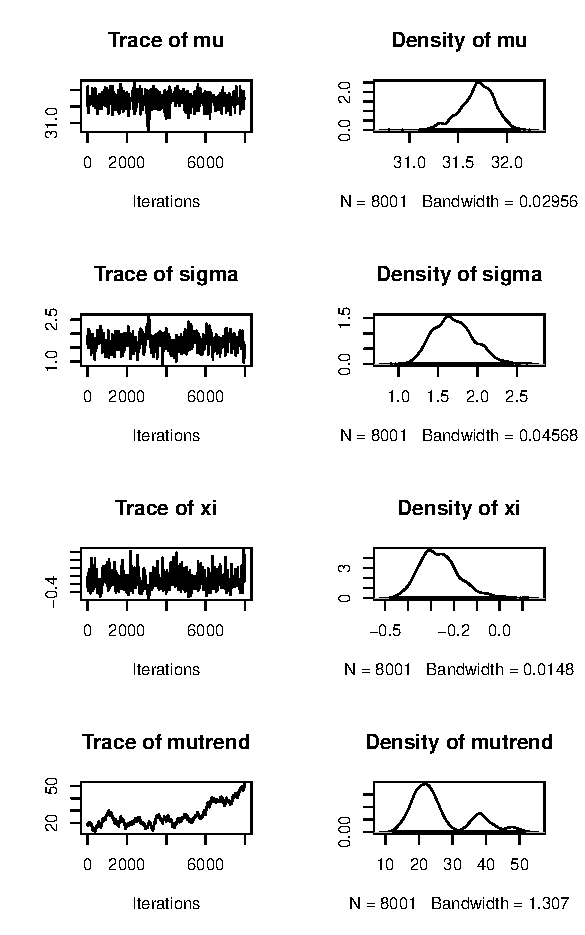
\includegraphics[scale = 0.4]{bay.pdf}
\vspace{-1.5cm} \hspace{-.6cm}
	\end{column}
\vspace{-1.5cm}
	\end{columns}
\end{frame}

\begin{frame}{Mixture Models} 
	
	\begin{columns}[T]
		\begin{column}{.5\textwidth}
		
	%\textbf{Mixture models} allows to 
	\begin{block}{Mixture Models rely on 2 separate}
	\begin{itemize}
		\item[$\bullet$] \underline{\textbf{Bulk} model} : \small  below threshold, either parametric or non(semi)parametric
	\normalsize	\item[$\bullet$]\underline{\textbf{Excess} model} : \small above threshold, is of the GPD family
	\end{itemize}
	
	\end{block}
	\vspace{-.15cm}
$\Rightarrow$ Put together to obtain full distribution of the data : improve fitting, asses threshold uncertainty, ...
		\vspace{2.5mm}
	
		$\boxed{  
		 f(x)=(1-\phi_u)\cdot \boldsymbol{b_t(x)}+\phi_u\cdot \boldsymbol{g(x)},}$ \\ \vspace{.05cm}
	\scriptsize	$\phi_u\ =\ \text{Pr}(X>u) \ \text{is the \emph{"tail fraction".}}$
	\normalsize
	\vspace{.2cm}
	 \begin{itemize}
	 	\item[$\bullet$] Main R package is \texttt{evmix}
	 	\item[$\bullet$] From now, we did not obtained relevant results
	 			\vspace{-.1cm}
	\small   \item\item[{\fontfamily{cyklop}\fontsize{6}{6}\selectfont \boxed{\textit{?}}}] In theory, model seems very interesting... But in practice, is it really worth it?
	 \end{itemize}
	 		\end{column}
	 		\hspace{2pt} \hspace{2pt}
	 \begin{column}{.55\textwidth}
	 	

	 	\begin{figure}	
%	\includepdf[pages = {16}, width=\textwidth]{mac.pdf}
	  \includegraphics[trim={4.5cm 3.3cm 
	  	5cm 8.3cm},clip,width=2.3in,height=3in, page = 16]{mac.pdf}
\vspace{-4.5mm}
\caption{\fontsize{1}{1}\selectfont
\textcolor{MidnightBlue}{\emph{\texttt{Figure}}} of models taken from \textcolor{JungleGreen}{\cite{scarrott_review_2012}}}
	\end{figure}
	
\end{column}
	\end{columns}
\end{frame}


\section{"Conclusions"}

\begin{frame}{Temporary Conclusions}
	\underline{What I have done : }
	\begin{itemize}
		\item[$\blacktriangleright$] Literature review and description of most concepts from univariate EVT
		\item[$\blacktriangleright$] \texttt{R} implementation of the data (still to enhance?) : 
		\begin{itemize} 	\fontsize{7}{7}\selectfont
			\item[$\blacktriangleright$] preprocessing of data,  methods from the various packages in EVT + comparisons,  (re)building of functions
			\item[$\blacktriangleright$] Stationary + non-stationary analysis, variable threshold
			\item[$\vartriangleright$] Bayesian analysis, Neural Network
		\end{itemize}
		\item[$\vartriangleright$] Understanding concept of Mixture Models in EVT
		\item[$\vartriangleright$] Bootstrap to improve accuracy or to compare models
	\end{itemize}
	
\underline{Still to do :}
\vspace{-.1cm}
\begin{itemize}
	\item[$\vartriangleright$] Aggregate used concepts into a smooth goal-oriented final document  
		\vspace{-.3cm}
\item\item[{\fontfamily{cyklop}\fontsize{6}{6}\selectfont \boxed{\textit{?}}}] Build other simulated data in order to make reliable comparisons of the available models.
	\end{itemize}
	
	
\end{frame}

\appendix
	\thispagestyle{empty}
\begin{frame}[allowframebreaks]
\bibliographystyle{apalike}
\bibliography{zotero.bib}
\end{frame}
	\thispagestyle{empty}
\end{document}